\documentclass[a4paper]{article}

% Use the postscript times font!
\usepackage{times}
\usepackage{soul}
\usepackage{color}
\usepackage[hyphens]{url}
\usepackage[hidelinks]{hyperref}
\usepackage[utf8]{inputenc}
\usepackage[small]{caption}
\usepackage{graphicx}
\usepackage{subcaption}
\usepackage{amsmath,amssymb}
\usepackage{booktabs}
\usepackage{cleveref}
\usepackage{multirow}
\usepackage{caption}
\usepackage{subcaption}
\usepackage[a4paper, portrait, margin=1in]{geometry}
\urlstyle{same}

\usepackage{parskip}

\usepackage{listings}
\usepackage{xcolor}
\definecolor{codegreen}{rgb}{0,0.6,0}
\definecolor{codegray}{rgb}{0.5,0.5,0.5}
\definecolor{codepurple}{rgb}{0.58,0,0.82}
\definecolor{backcolour}{rgb}{0.95,0.95,0.92}

\lstdefinestyle{mystyle}{
    backgroundcolor=\color{backcolour},   
    commentstyle=\color{codegreen},
    keywordstyle=\color{magenta},
    numberstyle=\tiny\color{codegray},
    stringstyle=\color{codepurple},
    basicstyle=\ttfamily\footnotesize,
    breakatwhitespace=false,         
    breaklines=true,                 
    captionpos=b,                    
    keepspaces=true,                 
    numbers=left,                    
    numbersep=5pt,                  
    showspaces=false,                
    showstringspaces=false,
    showtabs=false,                  
    tabsize=2
}
\lstset{style=mystyle}
\lstset{language=Python}

\newlength{\twosubht}
\newsavebox{\twosubbox}

% the following package is optional:
%\usepackage{latexsym} 

\title{CS6735 Programming Project Report}

\makeatletter
\renewcommand\@date{{%
  \vspace{-\baselineskip}%
  \large\centering
  \begin{tabular}{@{}c@{}}
    Ethan Garnier\textsuperscript{1} \\
    \normalsize ethan.garnier78@unb.ca 
  \end{tabular}%
  \hspace{3mm}
  \begin{tabular}{@{}c@{}}
    Matthew Tidd\textsuperscript{2} \\
    \normalsize mtidd2@unb.ca
  \end{tabular}
  \hspace{3mm}
  \begin{tabular}{@{}c@{}}
    Minh Nguyen\textsuperscript{2} \\
    \normalsize mnguyen6@unb.ca
  \end{tabular}
  
  \bigskip

  \textsuperscript{1}Department of Electrical and Computer Engineering, UNB\par
  \textsuperscript{2}Department of Mechanical Engineering, UNB

  \bigskip

  \today
}}
\makeatother

\begin{document}

\maketitle

\begin{abstract}
    In the field of Artificial Intelligence and Machine Learning, it can be very easy for the complexities of learning models to be obscured away behind the black boxes that are machine learning libraries. Despite the ease of use by which these libraries present, they do not always provide a complete understanding of how the learning is taking place. To truly grasp and take advantage of machine learning, one must understand the inner workings of the learning models being applied. This assignment saw students manually implement three machine learning models to truly test their understanding of these models and how they function. These models were: Adaboost with an ID3 weak base learner, an Artificial Neural Network with back-propagation, and Naïve Bayes. In addition to manually implementing these three learning models from scratch, two machine learning problems were solved using pre-existing machine learning libraries. These problems included developing a Deep Fully-Connected Feed-Forward Artificial Neural Network, and a Convolutional Neural Network to be trained and tested on the MNIST dataset of handwritten digits.
\end{abstract}

\newpage

\section{Introduction}

\section{Naive Bayes for Car Evaluation}
In this section of the report, the team implemented a Naive Bayes (NB) classifier from scratch and investigated the performance of the algorithm. In essence, NB classifiers are a machine learning model that learns the probability distribution in the training data under the naive assumption that the data features are conditionally independent. Therefore, the algorithm is a simple implementation of Bayesian networks. This section starts with a review of the theory and mechanism of NB classifiers, followed by a description of the car evaluation dataset, NB classifier implementation, finally the results and discussion of results.

\subsection{Naive Bayes Classifier Theory}

To assist in the formulation of an NB classifier, assume a dataset that contains training instances, each defined by a feature vector of \textit{n} features $\vec{x}=(x_1, x_2, \cdots x_n)$ and a class value, $C$. NB classifiers are ideal when working with categorical features. The NB classifier is trained to classify a test example based on its feature values and the probability distribution provided in the training set. NB classifier operates based on Bayes theorem, formulated as:

\begin{equation} \label{eq:Bayes_theorem}
    p(C_k|\vec{x}) = \frac{p(C_k)p(\vec{x}|C_k)}{p(\vec{x})}
\end{equation}

where $p(C_k|\vec x)$ represents the probability of a class, $C_k$, given the input features, $p(C_k)$ is the prior probability of the class from the data set, $p(\vec x|C_k)$ is the likelihood of the feature vector given the class, and $p(\vec x)$ is the evidence probability. Bayes Theorem plays an important role in Bayes classifiers since it allows for the classification of new data samples by leveraging the known distribution from the dataset. The left expression in \cref{eq:Bayes_theorem} is the quantity of interest since one can determine the probability of each class given the feature vector $\vec {x}$ and classify the instance as the class with the highest probability. The probability of each class given a data sample has the same denominator, $p(\vec x)$, as a normalizing factor. This can be simplified when considering the relative probabilities among classes.

\begin{equation} \label{eq:Bayes_theorem_simplified}
    p(C_k|\vec{x}) \propto p(C_k)p(\vec{x}|C_k)
\end{equation}

However, the left expression is challenging to obtain compared to the probabilities in the right expression. The prior probability $p(C_k)$ is the proportion of training samples with the class $C_k$ in the dataset. The likelihood $p(\vec x|C_k)$ is the number of samples of class $C_k$ with the features of $\vec x$. However, the curse of dimensionality presents the biggest drawback of this method. Computation time increases exponentially with the number of features. This quantity is further simplified in Naive Bayes with the assumption of conditional probability. Under this assumption, the features are independent when given the class label. Mathematically, this assumption simplifies the joint probability of the likelihood, $p(\vec x|C_k)$, to the product of individual conditional probabilities as:

\begin{equation}
\begin{aligned}
    p(\vec x|C_k) &= p(x_1, x_2 , ... , x_n|C_k) = p(x_1|C_k)\times p(x_2|C_k) \times ... p(x_n|C_k) \\
    p(\vec x|C_k) &= \prod_{i=1}^n p(x_i|C_k)
\end{aligned}
\end{equation}

With this simplifying assumption, computation time only increases linearly with the number of features compared to the joint probability calculation. The expression in \cref{eq:Bayes_theorem_simplified} is then further simplified as:

\begin{equation}
     p(C_k|\vec{x}) \, \propto \, p(C_k) \prod_{i=1}^n p(x_i|C_k)
\end{equation}


\subsection{Implementation of Naive Bayes Classifier}

\subsubsection{Platform} \label{subsubsec:platform}

A Naive Bayes Classifier algorithm was developed using Python in the Visual Studio Code development environment. The code was implemented in the form of code blocks in a Jypyter notebook and versioning was handled using Git to the main project repository. The Naive Bayes classifier and the helper functions were developed from scratch and employed Python built-in libraries for efficient numerical handling. More specifically

\begin{itemize}
    \item \lstinline{ucimlrepo} - for importing the car dataset
    \item \lstinline{pandas} - for working with data frames and related tasks, such as statistics, sample counting, ...
    \item \lstinline{sklearn} - for splitting the dataset into train and test set and evaluation scoring metrics 
    \item \lstinline{matplotlib} - for visualizing for 
    \item \lstinline{collection} - to import the \lstinline{defaultdict} construct to define empty nested dictionary for the individual conditional probabilities
\end{itemize}

\subsubsection{Dataset Description}
From the data discovery steps, the original dataset contains 1727 instances. Each instance has six categorical features - buying price, maintenance cost, number of doors, passenger capacity, size of the lug boot, and safety - encoded as 

\begin{itemize}
    \item buying: The buying price has 4 categories - low, med, high, and high
    \item  maint: The maintenance price has the similar 4 categories
    \item doors: The number of doors has 4 categories - 2, 3, 4, and 5more
    \item person: The number of passenger capacity has 3 categories - 2, 4, and more
    \item lug\_boot: The size of luggage boot has 3 categories - small, med, and big
    \item safety: The estimated car safety has 3 categories - low, med, and high
\end{itemize}

From these categorical features, the team must create a Naive Bayes classifier to classify the car as unacceptable, acceptable, good, or very good. From the training dataset, the probability distribution of the output classes is given as:

\begin{itemize}
    \item unacc class with 1,210 samples
    \item acc class with 384 samples
    \item good class with 69 samples
    \item good class with 65 samples
\end{itemize}

This seems to be an imbalanced dataset and will have a strong effect on the performance of the NB classifier since the \lstinline{unacc} class will have a much larger prior probability. Furthermore, since NB classifiers depend on the feature conditional probability $p(x_i|C_k)$. The conditional probability of the minority classes is inaccurate due to insufficient knowledge from the few samples of the class, such as \lstinline{good} or \lstinline{vgood}. In the end, even if the algorithm has high accuracy, it might still not be dependable as it might classify all cars as either \lstinline{unacc} or \lstinline{acc}. Therefore, precision, recall, and F1-score of the minority classes are other methods to provide insight into the model performance.

From a brief review, there are two main methods for handling an imbalanced dataset - data resampling and weighting factor.
The method of dataset resampling works by either upsampling the minority classes or downsampling the majority classes. As the name suggests, downsampling discards several instances of the majority class in the dataset, effectively causing a loss of information. This method is more applicable to large datasets with mild imbalances. On the other hand, upsampling techniques can duplicate or generate synthetic data from the existing minority instances, effectively boosting the prior probability of these classes. Duplicating existing data points is the simplest upsampling method, where we assume that the existing instances can capture the actual distribution of real-world data. However, once this assumption is violated, the classifier would overfit the existing data and generalize poorly to future testing data. A more advanced upsampling method is the synthetic minority oversampling technique, or SMOTE. This method works by synthesizing data points from the existing minority instances. The technique generates data points using K nearest neighbor, thus is only applicable for numerical data. Nonetheless, minority upsampling via duplication will be implemented and evaluated in this report.

The second method for handling imbalanced datasets is using weighting factors. This method essentially boost the prior probability, or the importance, of the underrepresented set. As a result of this, the classifier will have a higher chance to categorize instances as \lstinline{good} or \lstinline{vgood} depending on the feature vector.

\subsubsection{Program Structure}
The first section of the \lstinline{naivebayes.ipynb} notebook imports the dataset from the source and the necessary libraries for data handling (as detailed in \ref{subsubsec:platform}). The \lstinline{ucimlrepo} library has the \lstinline{fetch_ucirepo} function to load the dataset when given the dataset id. This function was used for importing the car evaluation dataset into a feature and a label data frame before they were split into the train and test data frames. The train test split was set as 90-10 and this parameter was not further experimented in this report.

To explore some statistics of the data frame and some data instances, the \lstinline{describe} and \lstinline{sample} functions were used. The first method reported several statistics for each feature, such as the number of instances, the number of unique feature values, the mode, and the frequency of the mode. The \lstinline{sample} function shows random samples from the dataset and displays the unique values of each feature. The team also investigated the number of training instances in each class to highlight the imbalance in the dataset.

The functional implementation of a Naive Bayes classifier consists of several subsections for defining helper functions, evaluating the prior and conditional probability, and the NB classifier implementation and evaluation. The first helper function, \lstinline{find_prior_probs()}, returns the prior probability of each classes in the dataset. The function takes the training data frame, the name of the label column, and a \lstinline{minority_class} dictionary containing user-defined weighting factors. The function extracts the list of unique label values, iterates through each label and counts the number of the labels in the training dataset, and divides this by the total number of training data to obtain the prior probability. If the class has a weighting factor defined in the \lstinline{minority_class} input argument, its prior probability is modified accordingly. The class name and prior probability are returned as a dictionary.

The function find\_cond\_probs was defined to determine the conditional probability of each feature when given the class. The information was stored in the format of class values \> feature names \> feature values \> feature conditional probability in a 3-tier Python library. An example of this nested structure is shown in \autoref{feature_conditional_prob_nested_dict}

\begin{lstlisting}[language=Python, label={feature_conditional_prob_nested_dict}, caption={Pseudo-code of the nested dictionary structure containing the conditional probabilities for P(feature value|class)}]
# level 1 - class values-feature name key-value pair
# level 2 - feature name-feature value key-value pair
# level 3 - feature value-conditional probability key-value pair
feature_cond_probs = {                    
  "unacc" : {                             
    "buying": {                           
      "low": P(buying=low|class_value=unacc),
      "medium": P(buying=medium|class_value=unacc),
      ...
    }
    "maint": {
      "low": P(maint=low|class_value=unacc),
      "medium": P(maint=medium|class_value=unacc),
      ...
    }
  }
}
\end{lstlisting}

To access the conditional probabilty P(feature\_name==feature\_value|class==class\_value) for Naive Bayes algorithm, we would index into the dictionary as feature\_cond\_probs[class\_value][feature\_name][feature\_value]. The function populates all the conditional probability values feature-by-feature. For every feature, it iterates through the available classes, find the subset of the training dataset with that class, and find the probability of each feature value in the subset. In other words, the function divides the number of instance with both the current feature value and the current class value by the number of instances with the current class value according to the product rule of probability

\begin{equation}
  \begin{aligned}
    P(feature\_value \cap class\_value) &= P(feature\_value|class\_value)P(class\_value)\\
    P(feature\_value|class\_value) &= \frac{\text{\# instances with feature\_value \& class\_value}}{\text{\# instances with the class\_value}}
  \end{aligned} 
\end{equation}

With these two functions, we can find the prior proability of the classes and the conditional probability of the feature values when given the class values from the dataset. As the dataset is highly imbalanced with the \lstinline{good} and \lstinline{vgood} minority classs, the prior probability of these classes were boosted by different weighting factors. A \lstinline{naive_bayes_classifier()} function was then defined to classify future testing instances given these probabilities. Classification is done by first extracting the prior probability $p(C_k)$ of each class k as shown in line 13 of \autoref{code:naive_bayes_classifier}. The function then cumulatively multiplies the individual conditional probability $p(x_i|C_k)$, where $x_i$ is the feature values of the instance to find the relative conditional probabilities of the instance (line 16-17 of \autoref{code:naive_bayes_classifier}). For each testing instance, the function finds the class probabilities and categorizes the instance as the class with the highest probability (line 20 in \autoref{code:naive_bayes_classifier}). The classifier function can takes an array of testing instances as a list of feature vectors. At the end, the function returns a list of class predictions for the given instances.

\begin{lstlisting} [language=Python, label={code:naive_bayes_classifier}, caption={Implementation of a Naive Bayes Classifier}]
  def naive_bayes_classifier(prior_probs, cond_probs, instances):
    # Get the list of classes (from the cond_probs structures)
    classes = []
    for item in cond_probs.items():
        classes.append(item[0])

    # List of empty dictionaries to store the class probabilities of each instance
    class_probs = [{}] * len(instances)                                        
    
    for index, instance in enumerate(instances):
        # Iterate over each class to find the prior probability 
        for c in classes:
            class_probs[index][c] = prior_probs[c]                  # p(class==c)

            # Iterate over instance features to accumulate conditional probabilties
            for feature,value in instance.items():
                class_probs[index][c] *= max(cond_probs[c][feature][value],1e-6)       
                # In case of zero probability, use a small number
        
        class_probs[index] = max(class_probs[index], key=class_probs[index].get)
  return class_probs
\end{lstlisting}

The NB classifier was then used to make predictions on the samples from the test set. The test set was first converted from a data frame to a list of Python dictionaries, each representing the feature vector of an instance. The list of dictionaries are then passed into the classifier to produce a list of the prediction class. This list is then converted back into a pandas dataframe so that it can be concatenated to the original test set for label-prediction comparison. Random samples from the test set was displayed with the NB classifier prediction to show high similarity between the label and the prediction.

The team used several evaluation metrics for algorithm performance assessment. The first metric that came to mind is accuracy, given as:

\begin{equation}
  Accuracy = \frac{\text{Correct predictions}}{\text{Number of instances}}
\end{equation}

However, accuracy is not an indicative metric when making evaluation on an imbalanced dataset. If the there is an overwhelmingly majority class in the dataset, the model can have a high accuracy by classifying all instances as the majority class. Therefore, complementary metrics such as precision, recall, and F1-score were employed. 

\begin{subequations}
\begin{align}
  \text{Recall} &= \frac{\sum \text{True Positives}}{\sum \text{True Positive + False Negative}} = \frac{\text{\# correctly classified instances}}{\text{\# instances in the class}} \\
  \text{Precision} &= \frac{\sum \text{True Positives}}{\sum \text{True Positive + False Positive}} = \frac{\text{\# instances correctly classified as class } C_k}{\text{\# instances classified as class } C_k} \\
  \text{F1-score} &= \frac{\text{Precision}\cdot\text{Recall}}{\text{Precision}+\text{Recall}}
\end{align}
\end{subequations}

The recall metric has the same representation as accuracy, but it is the percentage of correctly classified instances in each class. Thefore, if the model misclassified every instances as the majority classes, the recall of minority classes will be low. On the other hand, precision reflects the quality of the positive prediction of the model. This metrics is important when the positive must be accurate. For example, precision will be low if the classifier categorizes unacc, acc, or vgood cars as good. Finally, the F1-score is a harmonized metric that combines both the recall and precision

Furthermore, the team used a confusion matrix as shown in \autoref{fig:NBCcm} to visualize the classifier performance.

\begin{figure} [h]
  \centering{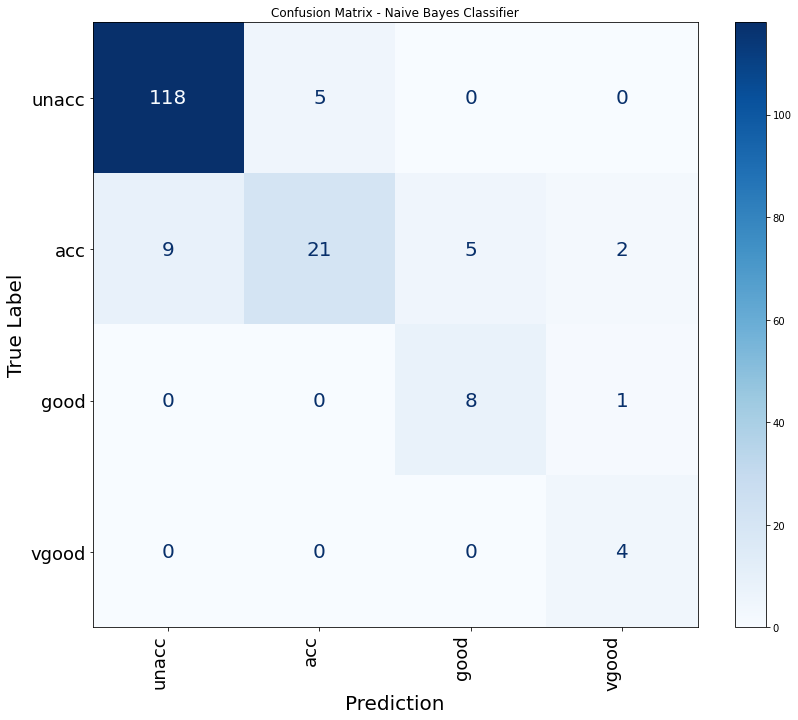
\includegraphics[scale=0.3]{../images/NBCcm.png}}
  \caption{Confusion matrix of the Naive Bayes classifier} 
  \label{fig:NBCcm}
\end{figure}


\subsection{Results and Discussion}
The results of the NB classifier, as quantified by the metrics outlined in the previous section, are reported here. In this section of the project, the weighting factor of the minority classes are varied to investigate their influence on the classification performance on the minority classes. Since the minority classes have similar distribution in the dataset, the same weighting factor was applied to both classes.

\subsubsection{Classifier with unmodified prior probability}
When there was no weighting factor to boost the prior probability of the \lstinline{good} and \lstinline{vgood} classes, it was expected that the model would predominantly classify testing instances as either \lstinline{unacc} or \lstinline{acc}. This was evident when the prior probability of each minority class was below 0.04 compared to $p(unacc)=0.699$ and $p(acc)=0.223$. 

The overall accuracy of this classifier was 86.71\%. The confusion matrix of this unmodified classifier is shown in \autoref{fig:NBCcm_unmodified}. 

\begin{figure} [h]
  \centering{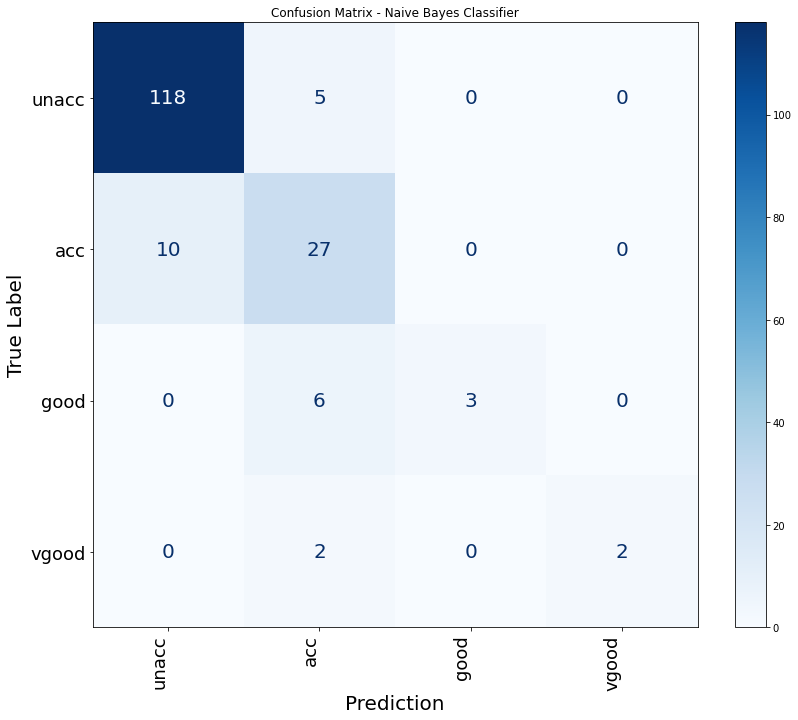
\includegraphics[scale=0.3]{../images/NBCcm_unmodified.png}}
  \caption{Confusion matrix of the Naive Bayes classifier with unmodified prior probabilities} 
  \label{fig:NBCcm_unmodified}
\end{figure}


The other metrics of the model are included in \autoref{tab:nb_performance_unmodified}. As expected, the classifier exhibit outstanding precision and recall for the majority class. However, these quantities are significantly lower for the other three classes. This was the result of the prior probability discrepancy and lack of adequate training data in the minority classes.
\begin{table}[ht]
  \centering
  \caption{Performance Metrics of the Unmodified Naive Bayes classifier}
  \label{tab:nb_performance_unmodified}
  \begin{tabular}{lcccc}
  \toprule
  \textbf{ } & \textbf{Precision} & \textbf{Recall} & \textbf{F1-score} \\
  \midrule
  unacc & 0.92 & 0.96 & 0.94\\
  acc  & 0.68 & 0.73 & 0.73\\
  good & 1.00 & \hl{0.33} & \hl{0.50}\\
  vgood & 1.00 & \hl{0.50} & \hl{0.67}\\
  \bottomrule
  \end{tabular}
\end{table}

\subsubsection{Classifier with a weighting factor of 5}
Compared to the unmodifed classifier, the accuracy improved to 87.86\% when incorporating a weighting factor of 5 on the prior probabilities of both the minority classes. \autoref{fig:NBCcm_5} shows the confusion matrix of this classifier, while the classifier recall, precision, and F1-score are included in \autoref{tab:nb_performance_5}. Compared to th previous confusion matrix, we observed a rightward shift in the prediction, where some \lstinline{acc} instances are classified as \lstinline{good} and \lstinline{vgood} and some instances previously misclassified as \lstinline{acc} are now correctly classified as the minority classes. Evident by \autoref{tab:nb_performance_5}, by increasing the importance of the minority class, the model achieved significantly better performance on the minority classes while only slightly reduce its previous performance in the \lstinline{acc} class.

\begin{figure} [h]
  \centering{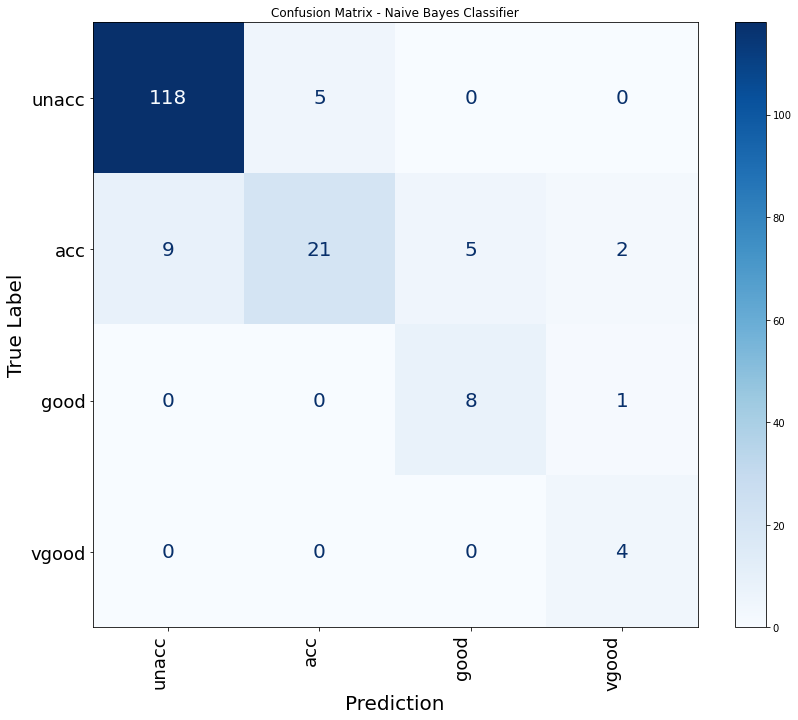
\includegraphics[scale=0.3]{../images/NBCcm_10.png}}
  \caption{Confusion matrix of the Naive Bayes classifier with a weighting factor of 5} 
  \label{fig:NBCcm_5}
\end{figure}

\begin{table}[ht]
  \centering
  \caption{Performance Metrics of the Unmodified Naive Bayes classifier}
  \label{tab:nb_performance_5}
  \begin{tabular}{lcccc}
  \toprule
  \textbf{ } & \textbf{Precision} & \textbf{Recall} & \textbf{F1-score} \\
  \midrule
  unacc & 0.93 & 0.96 & 0.94\\
  acc  & 0.81 & 0.59 & 0.69\\
  good & 0.67 & \hl{0.89} & \hl{0.76}\\
  vgood & 0.57 & \hl{1.00} & \hl{0.73}\\
  \bottomrule
  \end{tabular}
\end{table}


\subsubsection{Classifier with a weighting factor of 10}
The accuracy of the model was slightly improved to 87.28\% when a weighting factor of 10 was incorporated in the prior probability of both the \lstinline{good} and \lstinline{vgood} classes. The confusion matrix of the classifier is provided in \autoref{fig:NBCcm_10} while the classifier recall, precision, and F1-score are included in \autoref{tab:nb_performance_10}. In terms of the F1-score, this classifier had comparable performance for both the \lstinline{unacc} and \lstinline{acc} classes compared to the previous classifier with a slight decrease in performance for the \lstinline{good} class

\begin{figure} [h]
  \centering{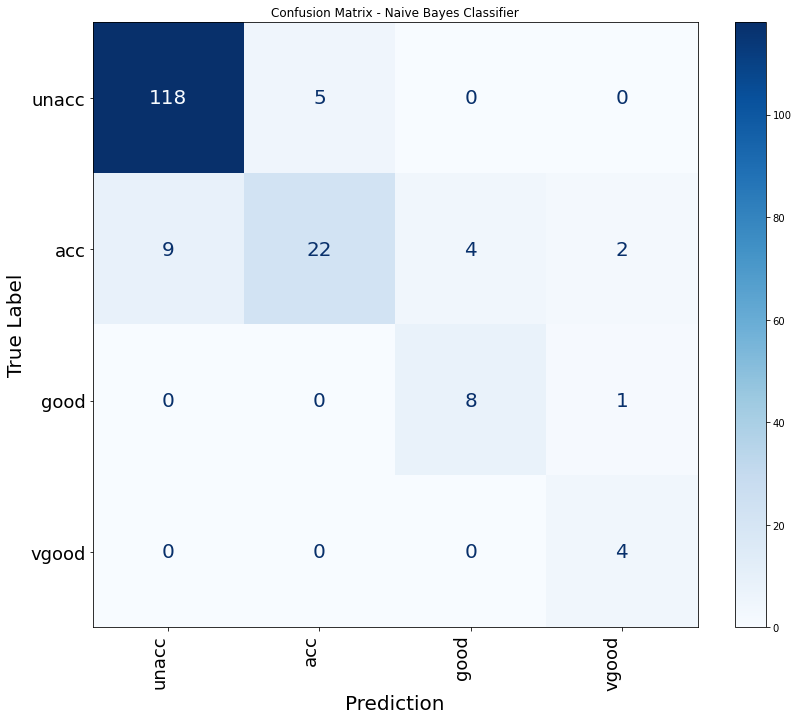
\includegraphics[scale=0.3]{../images/NBCcm_5.png}}
  \caption{Confusion matrix of the Naive Bayes classifier with a weighting factor of 10} 
  \label{fig:NBCcm_10}
\end{figure}


\begin{table}[ht]
  \centering
  \caption{Performance Metrics of the Unmodified Naive Bayes classifier}
  \label{tab:nb_performance_10}
  \begin{tabular}{lcccc}
  \toprule
  \textbf{ } & \textbf{Precision} & \textbf{Recall} & \textbf{F1-score} \\
  \midrule
  unacc & 0.93 & 0.96 & 0.94\\
  acc  & 0.81 & 0.57 & 0.67\\
  good & 0.62 & \hl{0.89} & \hl{0.73}\\
  vgood & 0.57 & \hl{1.00} & \hl{0.73}\\
  \bottomrule
  \end{tabular}
\end{table}

\subsection{Classifier with more prior probability adjustments} 
It was determined that there was no further imporvement in the model performance by further scaling the prior probability of the minority classes. At this point, more data is needed to fine tune and improve the performance of the model, especially for classifying the minority classes. Another methods was to manually fine tune the weighting factors of the \lstinline{acc} class. To test this, the weighting factors for the minority classes were fixed while the weighting factor of \lstinline{acc} was increased. The minority class weighting factor was fixed at 5 since this gave the best performance from previous sections, and the weighting factor of \lstinline{acc} was initialized at 1.25. The reason behind the conservative factor stems from the concern of misclassifying unacceptable cars as acceptable.

The accuracy of this model remained at 87.86\%. The confusion matrix of this classifier is shown in \autoref{fig:NBCcm_acc_class_weight_factor} and the performance metrics are summarized in \autoref{tab:nb_performance_1.25_5_5}.


\begin{figure}[h]
  % typeset
  \centering
  \subcaptionbox{\label{subfig:NBCcm_1.25_5_5}}{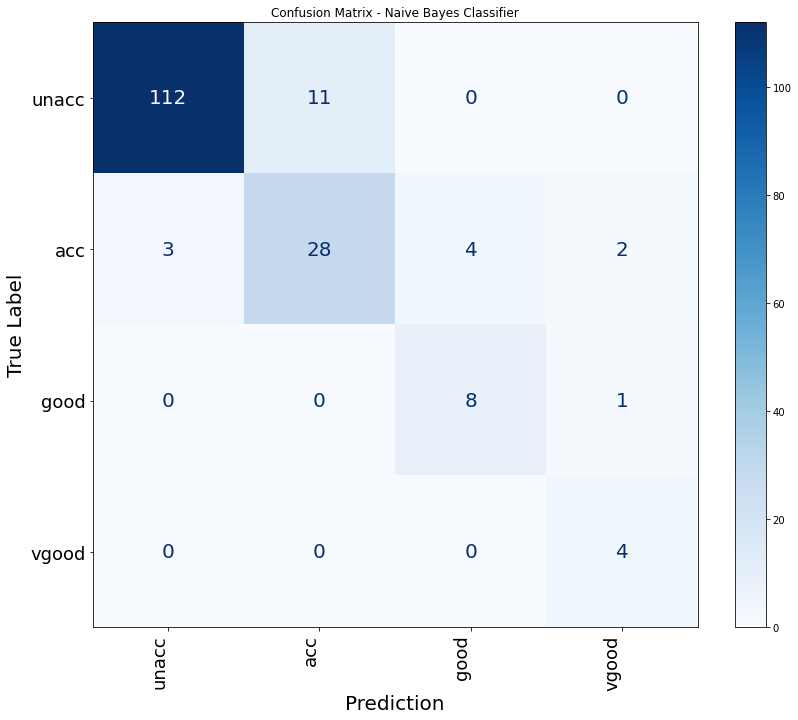
\includegraphics[width=0.48\textwidth]{../images/NBCcm_1.25_5_5.png}}
  \subcaptionbox{\label{subfig:NBCcm_1.5_5_5}}{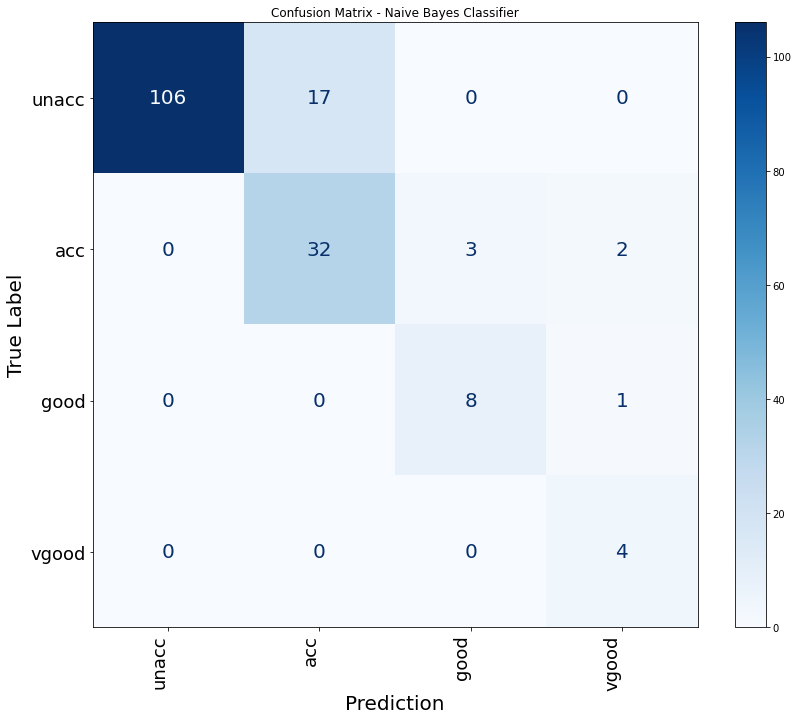
\includegraphics[width=0.48\textwidth]{../images/NBCcm_1.5_5_5.png}}
  \caption{Confusion matrix of the Naive Bayes classifier with a weighting factor of 5 for the minority classes and a weigting factor of 1.25 (left) and 1.5 (right) for the \lstinline{acc} class}
  \label{fig:NBCcm_acc_class_weight_factor}
\end{figure}

\begin{table}[ht]
  \centering
  \caption{Performance Metrics of the Naive Bayes classifier with mixed weighting factors}
  \label{tab:nb_performance_1.25_5_5}
  \begin{tabular}{|c|c|c|c|c|c|c|}

  \hline
  \centering
  \multirow{2}{*}{Class}    & \multicolumn{3}{c|}{Model 1 - Factor of 1.25}                     & \multicolumn{3}{c|}{Model 2 - Factor of 1.50} \\\cline{2-7} 
                            & \textbf{Precision}  & \textbf{Recall}   & \textbf{F1-score}       & \textbf{Precision}  & \textbf{Recall}   & \textbf{F1-score}\\
  \hline
  unacc                     & 0.97                & 0.91              & 0.94                    & 1.00                & 0.86              & 0.93\\
  acc                       & 0.72                & 0.76              & 0.74                    & 0.65                & 0.86              & 0.74\\
  good                      & 0.67                & \hl{0.89}         & \hl{0.76}               & 0.73                & \hl{0.89}         & \hl{0.80}\\
  vgood                     & 0.57                & \hl{1.00}         & \hl{0.73}               & 0.57                & \hl{1.00}         & \hl{0.73}\\
  % \bottomrule
  \hline
  \end{tabular}
\end{table}


It was found that by increasing this weighting factor to 1.25 and 1.5 achieve better F1-score for the \lstinline{acc} class and the minority classes. However, from the confusion matrix of these classifiers, more unacc instances are classified as acceptable. Depending on the severity of this misclassification in the real-world scenario (i.e., passing an unacceptable car with low safety and high buying price as acceptable), this improvement is not desireable.

% Bibliography/Reference Stuff
% \bibliographystyle{abbrv}
% \bibliography{main}
\end{document}